\documentclass{report}

\usepackage{amsmath, amsthm, amssymb, amsfonts}
\usepackage{thmtools}
\usepackage{graphicx}
\usepackage{subcaption}
\usepackage{setspace}
\usepackage{geometry}
\usepackage{float}
\usepackage{hyperref}
\usepackage[utf8]{inputenc}
\usepackage[english]{babel}
\usepackage{framed}
\usepackage[dvipsnames]{xcolor}
\usepackage{tcolorbox}
\usepackage{multicol}
\usepackage{minted}

\colorlet{LightGray}{White!90!Periwinkle}
\colorlet{LightOrange}{Orange!15}
\colorlet{LightGreen}{Green!15}

\newcommand{\HRule}[1]{\rule{\linewidth}{#1}}

\declaretheoremstyle[name=Theorem,]{thmsty}
\declaretheorem[style=thmsty,numberwithin=section]{theorem}
\tcolorboxenvironment{theorem}{colback=LightGray}

\declaretheoremstyle[name=Proposition,]{prosty}
\declaretheorem[style=prosty,numberlike=theorem]{proposition}
\tcolorboxenvironment{proposition}{colback=LightOrange}

\declaretheoremstyle[name=Principle,]{prcpsty}
\declaretheorem[style=prcpsty,numberlike=theorem]{principle}
\tcolorboxenvironment{principle}{colback=LightGreen}

\setstretch{1.2}
\geometry{
    textheight=9in,
    textwidth=5.5in,
    top=1in,
    headheight=12pt,
    headsep=25pt,
    footskip=30pt
}

% ------------------------------------------------------------------------------
\tcbset{
    sharp corners,
    colback = white,
    before skip = 0.2cm,    % add extra space before the box
    after skip = 0.5cm      % add extra space after the box
}                           % setting global options for tcolorbox

\definecolor{main}{HTML}{5989cf}    % setting main color to be used
\definecolor{sub}{HTML}{cde4ff}     % setting sub color to be used

\newtcolorbox{boxH}{
    colback = sub, 
    colframe = main, 
    boxrule = 0pt, 
    leftrule = 6pt % left rule weight
}

\newcommand{\SubItem}[1]{
    {\setlength\itemindent{15pt} \item[-] #1}
}

% ------------------------------------------------------------------------------

\begin{document}

% ------------------------------------------------------------------------------
% Cover Page and ToC
% ------------------------------------------------------------------------------

\title{ \normalsize \textsc{}
		\\ [2.0cm]
		\HRule{1.5pt} \\
    \LARGE \textbf{\uppercase{Computer forensics and Cyber crime analysis}}
		\HRule{2.0pt} \\ [0.6cm] \LARGE{Thats a lot of words in the title} \vspace*{10\baselineskip}}
\date{}
\author{\textbf{Fabio Lorenzato}} 
		

\maketitle
\newpage

\tableofcontents
\newpage

% ------------------------------------------------------------------------------

\part{Legal part}
\chapter{Introduction}
Back in the days, it was really easy to analyze the communication between two people, because the
technology was easier and know, meaning that the technology is \textit{between us}. Nowadays the
technology is more \textit{about us}, for example we use AI for facial recognition. Another example
are the social network algorithms that track our activity online. This means that we use the
technology to be "analyzed" instead of using it only to communicate. Most likely, the technology
will be \textit{in us}, which not only means robotics, but also be more integrated with human
beings.\\
In those scenarios, computer forensics became more complex, having to take in account no only the
quality of data(ie: a voice call), but also the quantity, which makes mistakes more likely to happen
in some instances. Another aspect of computer forensics will be to discern what is human from what
is a machine(ie: deep fakes, generative ai), and in particular where the liability lies.
Furthermore, it is necessary to handle the legal aspect of different countries, which is quite
difficult because of natural language limitations. An ideal solution would be to translate laws in
code, which is basically impossible, so we can approximate this solution with \textbf{legal design}
This has still to deal with two issues, which are information overloading(too much information), and
the fact that laws are written by lawyers for lawyers, which makes them difficult to understand.\\
Another aspect to consider is the GDPR, and the still to come AI act, for example the article 22
prevents automatic systems to make decisions having legal weight without the control of a human. An
example of this is the Lex Machina framework, which was able to predict the decisions of the judges
via ML methodologies, which was banned because it could influence the decisions of people and
judges. After all, false positives in digital forensics \textbf{can change people lives}.

\chapter{Foundations of digital forensics}
First of all, lets define what can be considered digital evidence.
There are many definition but the one that is most commonly used,and
the preferred one at the exam, is:
\begin{boxH}
  \textbf{Digital evidence} is \textit{any} information of evidential
  value whether memorized or sent in a \textbf{digital format}.
\end{boxH}
Digital evidence has some defining characteristics: it is invisible to
the untrained eye (it usually not simple to find), it may need to be
interpreted by a specialist, it may be altered or destroyed trough
normal use and it can be copied without limits (you must always work
on a copy to avoid tampering evidence).

Digital evidence, to be admissible in court, must have some
properties:
\begin{itemize}
  \item \textbf{Authenticity}: avoid any digital evidence
    \textbf{tampering}. Only certified formats should be used.
  \item \textbf{Reliable and believable}: the evidence must be redly
    \textbf{understandable} to the judge. Sometimes a report is not
    available to explain the evidence, so it must be self-explanatory.
  \item \textbf{Proportional}: \textbf{respect} fundamental
    \textbf{rights} of parties affected by the measure
  \item \textbf{Admissible}: \textbf{compliant with law} and best
    practices(admissible in court). One thing is to have evidence, the
    other is to have it admissible in court, and that's not always the
    case.
\end{itemize}

There are three main kinds of digital evidence:
\begin{itemize}
  \item \textbf{Created by man}: any piece of digital data that is the
    result of a step or action taken by a human person. Of those,
    there are two types:
    \begin{itemize}
      \item \textbf{Human to human}, such as an email
      \item \textbf{Human to machine}, such as a file saved on a disk
    \end{itemize}
  \item \textbf{Created independently by the computer}: any piece of
    digital data that is the result of the processing of data carried
    out by a software in accordance with a specific algorithm and
    without human intervention (e.g. telephone records or Internet
    Service Provider logs)
  \item \textbf{Created by both man and the computer}: an electronic
    spreadsheet where data is entered by the human, while the computer
    works out the result.
\end{itemize}

Lets now define what digital forensics is:
\begin{boxH}
  \textbf{Digital forensics} is the process of getting hold of
  evidence without modifying the IT system in which the evidence is
  found, ensure that the evidence acquired in another medium is
  identical to the original and analyze the evidence without modifying 
  it.
\end{boxH}

\subsubsection{The "Big Five" of digital forensics}
There are some principle that are to be followed during digital
forensics:
\begin{itemize}
  \item \textbf{Data Integrity}: No action taken should change
    electronic devices or media, which may subsequently be relied upon
    in court. 
  \item \textbf{Chain of Custody}: An audit trail of all actions taken
    when handling electronic evidence should be created and preserved. 
  \item \textbf{Specialist Support} If investigations involving search
    and seizure of electronic evidence it may be necessary to consult
    external specialists. 
  \item \textbf{Appropriate Training}: First responders must be
    appropriately trained to be able to search for and seize
    electronic evidence if no experts are available at the scene. 
  \item \textbf{Legality}: The person and agency in charge of the case
    are responsible for ensuring that the law and the above listed
    principles are adhered to. 
\end{itemize}

\section{Digital Investigation Procedure}
Digital investigation is carried out in many steps.
\subsection{Identify the Suspect}
The first phase is also the most difficult one, because there are many
tools to be anonymous in the internet.
The general approach to this phase is the following:
\begin{enumerate}
  \item An investigator receives a \textbf{complaint} by a victim of
    \textbf{cybercrime} or detect an illegal content on line. (OSINT
    can be used to detect illegal content)
  \item The investigator uses the Court System to compel the ISP to
    \textbf{reveal} a \textbf{physical location} that corresponds
    likely to the source of Network (\textbf{IP Address})
  \item Under a \textbf{warrant} (depending from the Jurisdiction) the location
    is searched and any computer or other device is seized
\end{enumerate}

But why the ISP has to cooperate and give away the IP address?
In the EU it is because \textbf{Data Retention Directive} 2006/24/EC,
that requires that all the data of the communication must be stored
for a certain amount of time, from 6 to 24 months. This directive was
unconstitutional in many countries,
\begin{boxH}
  \textbf{Data retention} (or data preservation) generally refers to
  the \textbf{storage} of call detail records (CDRs) of telephony and
  internet traffic and transaction data (IPDRs) by governments and
  commercial organizations
\end{boxH}
In any case data retention is usually a problem because there's no a
homogeneous law for data retention, mainly for privacy reasons.

Even if there's no data retention law, the request of user data
disclosure have been a lot in the past years have steadily increased,
because the processes have been automated, as you can also see from
figure \ref{fig:disclosure-req}.

\begin{figure}[H]
  \centering
  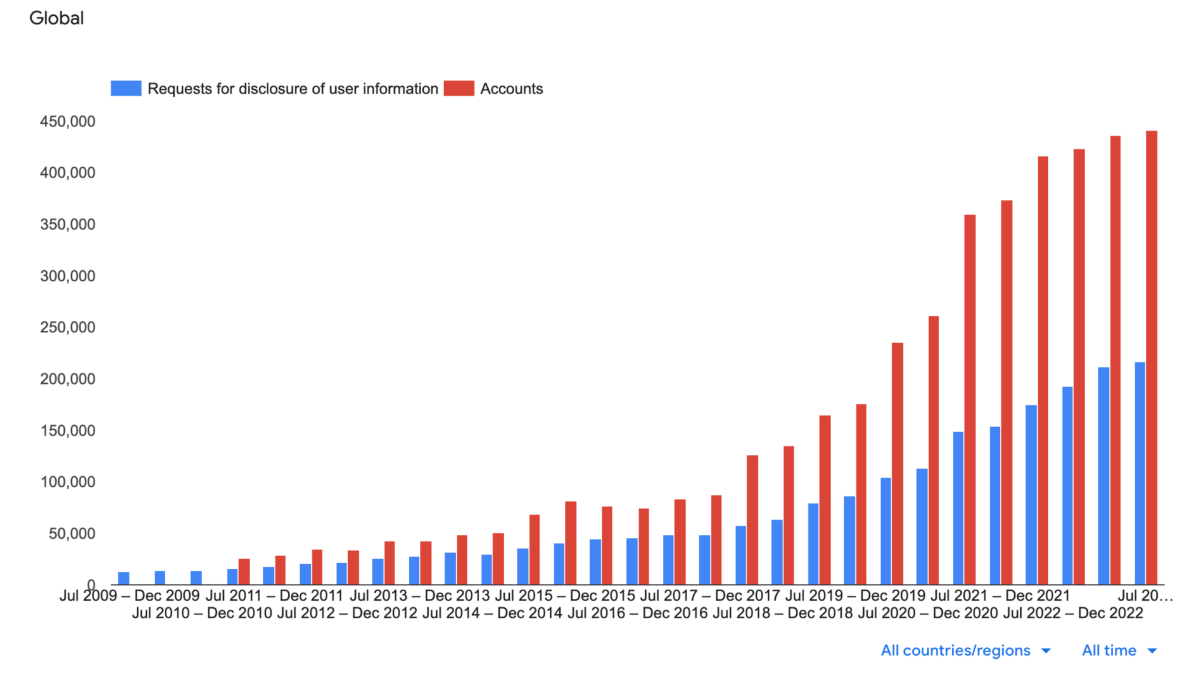
\includegraphics[scale=.4]{img/disclosure requests.png}
  \caption{Requests for user data disclosure during the years}
  \label{fig:disclosure-req}
\end{figure}
Another instrument that could be used to identify the suspect is the
\textbf{facial recognition}, that can be used only for terrorism
situations, but not in a systematic way.
\subsection{Detecting and Seizing Digital Evidence}
Anyone wanting to seize and validate digital/electronic evidences
(content of an e-mail or an entire hard-disk) has to respect two
fundamental \textbf{rules}: Bit-Stream Copy and Hash Function.
\subsubsection{Bit-Stream Copy}
\begin{boxH}
  A \textbf{bit-stream copy} can \textbf{clone} the \textbf{entire
  drive}.
\end{boxH}
It is a particular form of duplication in which the content of the
physical unit is read sequentially loading the minimum quantity of
data that can from time to time be directed, then recording it in the
same sequence on a standard binary file, generating a physical image
of the original medium.

\subsubsection{Hash Functions}
During the forensic analysis of modifiable media, the Hash 
guarantees the intangible nature of the data that it contains.
\begin{boxH}
  The Hash is a \textbf{one-way function}, by means of which a
  document of random length is converted into a limited and fixed
  length string.
\end{boxH}
This string represents a sort of ‘digital fingerprint’ of the non-
encrypted text, and is called the Hash Value or the Message Digest. If
the document is modified, even to the slightest extent, then the
fingerprint changes as well. In other words, by calculating and
recording the fingerprint, and then recalculating it, it can be shown
beyond all doubt whether the contents of the file, or the medium, have
been altered, even accidentally.\\

In any case we have two main problems while acquiring data: encryption
and jurisdiction. After all, the ISP, TELECO or even a bank does have
to cooperate and give out the data. Another big issue it the cloud
computing aspect, because the location of data is another big problem,
because it can be either:
\begin{itemize}
  \item \textbf{at rest}: does not reside on the device. 
  \item \textbf{in transit}: cannot be easily analysed because of
    encryption. 
  \item \textbf{in execution}: will be present only in the cloud
    instance
\end{itemize}
\textbf{Validation} of digital evidence is a very important step,
because it is the only way to prove that the evidence is authentic.
This is especially important for proof found on the internet. There
are some tools that can be used to validate digital evidence, such as
Web Forensics.\\
Another issue that has to be accouted for is the \textbf{chain of
custody}, that is the process of maintaining and documenting the
location and handling of evidence. After all, the bit is eternal, but
the storage medium is not.
\subsection{Validating Digital Evidence}
\subsection{Chain of Custody}
\subsection{Analysis of Digital Evidence}
\subsection{Presentation in Court}

\chapter{Cybercrime Convention}
Because this part it \textit{really boring} we will start with an
example.
\section{E-commerce on the Dark Web}
The Dark Web provides a \textbf{platform} for buyers and sellers to
engage in e-commerce transactions, often involving \textbf{illicit
goods and services}, like guns, fake documents etc.. This anonymous
marketplace operates with the same principles as traditional
e-commerce, but with heightened security and privacy measures to
conceal identities.\\
Vendors on the Dark Web offer a wide range of products, from drugs and
weapons to stolen data and hacking services. Buyers can browse
listings, read reviews, and complete purchases using cryptocurrencies,
all while maintaining a high degree of anonymity.
\subsection{Silk Road}
Silk Road, often referred to as the "eBay of drugs," was an
\textbf{online marketplace}that facilitated the sale of a wide range
of illegal substances, including narcotics and controlled substances.
At its peak in 2013, Silk Road had a reported annual revenue of \$89.7
million.
\begin{itemize}
  \item \textbf{Combining Tor, PGP, and Bitcoin}: Ross Ulbricht
    leveraged the anonymity of Tor, the encryption of PGP, and the
    decentralized nature of Bitcoin to create the Silk Road marketplace. 
  \item \textbf{Bitcoin-only Payments}: Silk Road required all
    transactions to be conducted using Bitcoin, providing an added layer
    of anonymity and making it harder to trace purchases.
  \item \textbf{User-friendly Interface}: Silk Road featured a well-designed
    interface that allowed users to easily navigate the site and leave
    feedback on their transactions.
  \item \textbf{Intermediary Role}: Silk Road acted as an intermediary
    between buyers and sellers, handling the payment process and
    logistics of shipping items purchased on the marketplace. This is
    one of the main sources of success of the platform.
\end{itemize}
At its peak, Silk Road had over 950,000 registered accounts, 1.2
million transactions, and nearly \$79 million in commissions. Ulbricht
was arrested in 2013 due to some critical mistakes, like using its
personal email to advertise the website and having counterfeit
documents delivered to his home address when he found out that he was
on investigation.\\
Ulbricht faced 7 key charges, including drug trafficking,
money laundering, and computer hacking, which were consolidated into 3
main counts against him and the trial ended in just 13 days with a
life sentence plus 180\$ million in damages.\\
What we can learn about this? First, the anonymity is really an issue
with ongoing investigations, but everyone can make mistakes, which
means that eventually, the law will catch up with you. Second,
everyone can create this kind of platform, which implies that is
necessary to solve the issue. For this purpose, cooperation is most
fundamental, and the Budapest Convention is the first step in this 
direction, by creating standards and protocols for international
cooperation in this field.

\section{Budapest Convention}
The Budapest Convention on Cybercrime is an international
\textbf{treaty} that aims to address the challenges posed by
cybercrime and promote cooperation among countries in combating these
offenses.
It has three main purposes:
\begin{itemize}
  \item Harmonizing national laws on cybercrime
  \item Improving investigative techniques
  \item Increasing international cooperation
\end{itemize}
In involves \textbf{68 countries}, including the United States,
Canada, and many European nations.
\begin{boxH}
  Keep in mind that the council of Europe and the European union are
  two different entities. The first one is able to invite entities
  that are outside of the latter one.
\end{boxH}

Some countries opposed to the convention like India, which has since
reconsidered, and Russia, which rejects it due to concerns about
sovereignty and refuses to cooperate too.\\
Other states has signed but no ratified (Ireland and South Africa),
which means that they are not bound by the convention(in this case is
just a principle declaration, without legal value).
\begin{boxH}
  The \textbf{difference} between signing and ratifying a treaty is
  that \textbf{signing} a treaty is a \textbf{preliminary step} that
  indicates a country's \textbf{intention to be bound} by the treaty,
  while \textbf{ratifying} a treaty is the \textbf{formal act} of
  \textbf{accepting} the treaty and agreeing to be bound by its terms.
  A country can sign a treaty without ratifying it, but it cannot
  ratify a treaty without signing it first.
\end{boxH}
The convention aims to help in the \textbf{fight against crimes} that
can only be committed through the \textbf{use of technology}, where
the devices are both the tool for committing the crime and the target
of the crime, and crimes where technology has been used to enhance
another crime, such as fraud. It \textbf{provides guidelines} for any
country \textbf{developing domestic laws on cybercrime}and serves as a
basis for international cooperation between parties to the convention
but was later expanded to cover other areas of crime, such as hate
crimes.
\subsection{Original key provisions}
The original convention was adopted in 2004 and covers:
\begin{itemize}
  \item the \textbf{criminalisation} of \textbf{conduct}, ranging from
    illegal access, data and systems interference to computer-related
    fraud and dissemination of child abuse material;
  \item \textbf{procedural powers} to \textbf{investigate cybercrime}
    and secure electronic evidence in relation to any crime;
  \item \textbf{efficient international cooperation} between parties.
\end{itemize}

Parties are members of the Cybercrime Convention Committee and:
\begin{itemize}
  \item \textbf{share information} and \textbf{experience};
  \item \textbf{assess implementation} of the convention;
  \item \textbf{interpret} the convention through \textbf{guidance
    notes}.
\end{itemize}

Of the 27 Member States, 26 have ratified the convention. Ireland
has signed but not yet ratified it.

\subsection{Additional Protocol 1(2006)}
This protocol extends the scope of the convention to cover xenophobic
and racist propaganda disseminated through computer systems, providing
more protection for victims.\\
It furthermore:
\begin{itemize}
  \item reinforces the legal framework through a set of guidelines for
    criminalising xenophobia and racist propaganda in cyberspace;
  \item enhances the ways and means for international cooperation in the
    investigation and prosecution of racist and xenophobic crimes online.
\end{itemize}

\subsection{Additional Protocol 2(2024)}
This protocol aims to further enhance international cooperation.\\
It addresses the particular challenge of \textbf{electronic evidence}
relating to cybercrime and other offences being held by service
providers in foreign jurisdictions, but with law enforcement powers
limited to national boundaries.\\
Its main features are:
\begin{itemize}
  \item a new \textbf{legal basis} permitting a \textbf{direct request
    to registrars} in other jurisdictions to obtain domain name
    registration information;
  \item a new \textbf{legal base} permitting \textbf{direct orders to
    service providers} in \textbf{other jurisdictions} to obtain
    subscriber information;
  \item \textbf{enhanced} means for \textbf{obtaining subscriber
    information} and \textbf{traffic data} through
    government-to-government cooperation;
  \item expedited \textbf{cooperation} in \textbf{emergency
    situations} including the use of joint investigation teams and
    joint investigations.
\end{itemize}

\subsection{New Global Cybercrime Treaty}
The Budapest Convention has been a model for other countries and 
regions in developing their own cybercrime laws and treaties.\\ 
The \textbf{United Nations} has also been working on a new global 
cybercrime treaty, which would build on the Budapest Convention and 
expand its scope to cover new forms of cybercrime and emerging 
technologies.\\
We will see it later on.

\section{Harmonization of national laws and international cooperation}
\subsection{International Cooperation Provisions}
This provision s based on a very simple principle.
\begin{boxH}
  Parties are to cooperate "to the \textbf{widest extent possible}" in
  investigating electronic evidence.
\end{boxH}
This is necessary because mutual assistance is often slow and can even
take months to complete(3 up to 6).  The Mutual assistance agreement(
thanks to the Cybercrime convention) allows for expedited requests
using "expedited means of communication", which means that, to an
expedited request, one must provide adequate levels of security and
authentication(eg. encrypted communication).\\
Furthermore, parties may share information without a formal request if
it would assist in investigations or help the receiving party with any
related offences.
\subsection{Mutual Assistance Provisions}
Procedural Powers for Assistance grant the ability to expedite the
preservation of stored computer data, as well as the disclosure of
traffic data. In addition, they allow for the real-time collection of
traffic data and the interception of content data. Assistance in these
matters is provided in accordance with domestic laws and applicable
treaties, subject to any reservations.\\
Article 23, which outlines the General Cooperation Principle,
emphasizes that mutual assistance should be offered to the widest
extent possible. This applies specifically to cyber-related offenses
and the collection of electronic evidence for any criminal offense.\\
However, there are restrictions to this cooperation. These limitations
may arise in cases related to extradition, mutual assistance in the
real-time collection of traffic data, and the interception of content
data.
\subsection{24/7 Network for Immediate Assistance}
Each party is required to designate a contact point that is available
24/7. The primary purpose of this contact point is to provide
immediate assistance in cybercrime investigations, legal proceedings,
or the collection of electronic evidence. This system is modeled after
the G8 network of contact points.\\
The goal of this provision is to expedite the processing of urgent
mutual assistance requests by overcoming delays associated with
traditional bureaucratic channels.

\section{Legal measures against computer-related fraud and forgery}
One of the main legal measures against computer-related fraud and 
forgery is the \textit{criminalization of Fraud and Computer-related
Forgery}.\\
The Convention mandates State Parties to criminalize specific
conducts, including fraud and forgery carried out through computer
systems. This includes digital document forgery and fraud involving
electronic data used for deceit or financial gain. 

\begin{boxH}
  Computer-related fraud involves using computers to gain economic
  benefits through deceit, while forgery includes altering or creating
  digital documents with the intent to mislead.
\end{boxH}

To effectively address these crimes, the Convention introduces
procedural law tools that allow for quicker and more effective
investigations.

For example, expedited preservation of volatile data and seizure of
information are crucial tools for gathering evidence in investigations
against digital fraud and forgery.

The Convention mandates that criminal justice authorities must be
able to use effective means, such as search and seizure, and access
stored data in computer systems, regardless of the type of crime
involved.
\subsection{Computer-Related Forgery}
Each Party shall adopt such legislative and other measures as may be
necessary to establish as criminal offences under its domestic law,
when committed intentionally and without right, the input,
\textbf{alteration, deletion, or suppression of computer data},
resulting in inauthentic data with the intent that it be considered or
acted upon for legal purposes as if it were authentic, regardless
whether or not the data is directly readable and intelligible. A Party
may require an intent to defraud, or similar dishonest intent, before
criminal liability attaches, this is to avoid criminalizing 
accidental behaviour because data alteration is so easy to do.
\subsection{Computer-Related Fraud}
Each Party shall adopt such legislative and other measures as may be
necessary to establish as criminal offences under its domestic law,
when committed intentionally and without right, the causing of a loss
of property to another person by:
\begin{enumerate}
  \item any input, alteration, deletion or suppression of computer data,
  \item any interference with the functioning of a computer system 
\end{enumerate}
with fraudulent or dishonest intent of procuring, without right, an
economic benefit for oneself or for another person.

\section{Procedural powers for law enforcement}
In the past years, we moved from a synopticon world (where the 
many watch the few) to a omnipticon world (where the many watch the
many). Think to a youtube video as an example. In this kind of world,
information control is much more difficult.

The main concern arising for private citizens, companies and public
administration using cloud technologies is not so much the possible
increase in "cyber" fraud or crime than the loss of control over one's
data.\\
This concern is not only for privacy reason, but for digital
investigation purposes.\\

All this is to say that we mainly lost control of our data, and this
is a big jurisdictional problem, because this is usually in the hands
of private companies, following their terms and conditions.
\subsection{Scope of Procedural Provisions (Article 14)}
Each Party must adopt legislative measures to define the powers and
procedures for specific criminal investigations or proceedings.

The provisions apply to offenses covered by the Convention, all other
offenses committed through computer systems, and all electronic
evidence related to any crime.
\subsection{Conditions and Safeguards (Article 15)}
The application of powers and procedures must ensure adequate
protection of human rights, following national law and international
conventions (e.g., European Convention on Human Rights).

Conditions and safeguards include judicial or independent supervision,
considering proportionality and the rights of third parties.
\subsection{Expedited Preservation of Stored Data (Article 16)}
Authorities must be able to order or obtain the rapid preservation
of specific computer data, particularly if there is reason to believe
that the data is vulnerable to deletion or modification.

This order may require the data's custodian to preserve the data for
up to 90 days, extendable as needed.

\subsection{Expedited Preservation and Disclosure of Traffic Data
(Article 17)}
To ensure data preservation, authorities can demand rapid disclosure
of traffic data to identify service providers and communication
pathways, even if multiple providers are involved in the transmission.

\subsection{Production Order (Article 18)}
Each Party shall adopt such legislative and other measures as
may be necessary to empower its competent authorities to
order:
\begin{enumerate}
  \item a person in its territory to submit specified computer data in
    that person’s possession or control, which is stored in a computer
    system or a computer-data storage medium; and
  \item a service provider offering its services in the territory of the
    Party to submit subscriber information relating to such services in
    that service provider’s possession or control.
\end{enumerate}

\subsection{Subscriber Information (Article 18)}

For the purpose of this article, the term \textit{subscriber
information} means any information contained in the form of computer
data or any other form that is held by a service provider, relating to
subscribers of its services other than traffic or content data, and by
which can be established:

\begin{itemize}
    \item[(a)] the type of communication service used, the technical
      provisions taken thereto, and the period of service;
    \item[(b)] the subscriber's identity, postal or geographic
      address, telephone and other access number, billing and payment
      information, available on the basis of the service agreement or
      arrangement;
    \item[(c)] any other information on the site of the installation
      of communication equipment, available on the basis of the
      service agreement or arrangement.
\end{itemize}

\subsection{Search and Seizure of Stored Computer Data (Article 19)}

Each Party shall adopt such legislative and other measures as may be
necessary to empower its competent authorities to search or similarly
access:

\begin{itemize}
    \item[(a)] a computer system or part of it and computer data
      stored therein
    \item[(b)] a computer-data storage medium in which computer data
      may be stored in its territory.
\end{itemize}

\subsection{Real-time Collection of Traffic Data (Article 20)}

Authorities can collect or record traffic data in real time, either
directly or by requiring service providers to assist in the
collection.

\subsection{Interception of Content Data (Article 21)}
For serious offenses, authorities may intercept or record the content
of specific communications in real time, either directly or through
the cooperation of service providers.

\begin{boxH}
  From all those you only need to remember article 25 and 29.
\end{boxH}

\subsection{Mutual Assistance (Article 25)}
The Parties shall afford one another mutual assistance to the widest
extent possible for the purpose of investigations or proceedings
concerning criminal offences related to computer systems and data, or
for the collection of evidence in electronic form of a criminal
offence.

The Parties shall afford one another mutual assistance to the widest
extent possible for the purpose of investigations or proceedings
concerning criminal offences related to computer systems and data, or
for the collection of evidence in electronic form of a criminal
offence.

\subsection{Expedited preservation of stored computer data (Article
29)}
A Party may request another Party to order or otherwise obtain the
expeditious preservation of data stored by means of a computer system,
located within the territory of that other Party and in respect of
which the requesting Party intends to submit a request for mutual
assistance for the search or similar access, seizure or similar
securing, or disclosure of the data.

\subsection{Expedited disclosure of preserved traffic data (Article
30)}
Where, in the course of the execution of a request made pursuant to
Article 29 to preserve traffic data concerning a specific
communication, the requested Party discovers that a service provider
in another State was involved in the transmission of the
communication, the requested Party shall expeditiously disclose to the
requesting Party a sufficient amount of traffic data to identify that
service provider and the path through which the communication was
transmitted.

\subsection{Article 32 of the Cybercrime Convention (Budapest 2001)}
A Party may, without the authorisation of another Party:
\begin{itemize}
  \item[(a)] access publicly available (open source) stored computer data, regardless of where the data is located geographically, or
  \item[(b)] access or receive, through a computer system in its territory, stored computer data located in another Party, if the Party obtains the lawful and voluntary consent of the
    person who has the lawful authority to disclose the data to the Party through that computer system.
\end{itemize}

\subsection{Additional Legal Framework}

Regulation (EU) 2023/1543 of the European Parliament and of the 
Council of 12 July 2023 on European Production Orders and European 
Preservation Orders for electronic evidence in criminal proceedings 
and for the execution of custodial sentences following criminal 
proceedings.


Directive (EU) 2023/1544 of the European Parliament and of the 
Council of 12 July 2023 laying down harmonised rules on the 
designation of designated establishments and the appointment of 
legal representatives for the purpose of gathering electronic 
evidence in criminal proceedings.

In order to apply the rules in a consistent manner and to provide 
time for implementation and compliance, the Regulation applies 
from 18 August 2026. The Directive must be transposed into the 
national laws of the EU Member States by 18 February 2026.


\chapter{Italian Law n. 48/2008}


The Budapest Convention on Cybercrime was issued by the Council of
Europe on November 23, 2001. 

\begin{boxH}
  Each country need to ratify a convenction (otherwise is only a
  general agreed principle, as in case of signature), therefore Italy
  ratified the it with Law n. 48 on March 18, 2008, which was
  published in the Official Gazette on April 4, 2008.
\end{boxH}

The ratification of the Budapest Convention by Italy through Law n.
48/2008 represents a critical step in modernizing the Italian legal
system to tackle cybercrime. This law aims to harmonize legal
standards across borders, emphasizing the importance of international
cooperation in addressing the rapidly evolving digital landscape.
However, challenges remain in adapting to rapid technological changes,
and continuous updates to legislative tools are necessary.

\section{Main Innovations Introduced by Italian Law n. 48/2008}

\begin{itemize}
    \item International harmonization of legislation to combat
      cybercrime.
    \item Reorganization of cybercrime offenses: amendments and
      integrations to the penal code, introducing new specific
      offenses.
    \item \textbf{Corporate Liability}: Extending liability under
      Legislative Decree 231/2001 to cover cybercrime offenses.
\end{itemize}

\section{Corporate Criminal Liability}

Italian Law n. 48/2008 extends corporate criminal liability to
offenses committed in the interest or for the benefit of the company,
as regulated by Legislative Decree 231/2001. 
\begin{boxH}
This applies to all legal entities, even foreign companies if the
offense is committed in Italy.
\end{boxH}

Manly, offences committed \textbf{in the interest} or \textbf{for the
benefit} of the company, and in most cases monetary fines,
interdictive sanctions  or publication of the sentence are applied to
the company.

The liability for the phisical persons lies to the person holding a
position of representation, management or direction or who exercise,
even if \textit{de facto}, management and control or a persons subject
to the control or monitoring activity of the Top Management.

The corporate liability, in Italy, is only applicable for some kinds
of crimes, such as tax offenses, money laundering, corruption, etc. In
case of corporate liaility, the company can demostrate to have a
compliance programm to ask for an exception, which is a set of
policies policies on the various topics, and demonstrate that all the
necessary measures have been taken to prevent the crime, and notheless
the crime has been committed.

\section{Further Innovations}

\begin{itemize}
    \item Establishment of a fund under the Ministry of the Interior
      to combat child pornography online.
    \item Updates to data retention laws, with reference to Directive
      2006/24/EC.
    \item Enhancement of international cooperation, especially
      concerning mutual assistance in cybercrime investigations.
    \item Acquisition of digital evidence: Updates to criminal
      procedure code for regulating the collection and use of digital
      evidence.
\end{itemize}

\section{Key Provisions and Their Implications for Digital Forensics}

\subsection{Major Procedural and Investigative Updates}

\subsubsection{International Cooperation}
The law enables the Ministry of the Interior or designated authorities to instruct internet and telecommunications providers to retain and protect traffic data for up to 90 days. This period can be extended to six months for specific investigative needs, but excludes the content of communications.

\subsubsection{Competence for Investigations and Prosecutions}
Cybercrime investigations and prosecutions are assigned to the Public Prosecutor’s Office at the Court of Appeal’s main district. This aims to improve coordination in cybercrime cases. However, initial issues arose due to the lack of transitional provisions for ongoing investigations, which were later addressed by Law n. 125 of July 2008.

\subsubsection{Service Providers' Role}
Service providers, including internet, telecommunications, and postal services, play a key role in combating cybercrime. Their responsibilities include:
\begin{itemize}
    \item Retention of traffic data and communication logs.
    \item Seizure of correspondence, including electronic communications, when linked to criminal investigations.
    \item Seizure of digital data, ensuring that original data is preserved while copies are made without modification.
\end{itemize}

\subsubsection{Legal Recognition of Computer Forensics}
The law introduces computer forensics as a significant element of investigative practices, with clear protocols for handling digital evidence. These practices will need continuous updates as technology evolves.

\subsection{Best Practices in Digital Evidence Handling}
The law advocates for "best practices" in digital evidence handling, emphasizing the importance of:
\begin{itemize}
    \item Acquiring evidence without altering the original device.
    \item Authenticating both the evidence and its digital copy.
    \item Ensuring that the examination process is repeatable.
    \item Maintaining impartiality in technical analysis.
\end{itemize}

\subsection{Email Seizures}
The law also includes provisions for seizing email communications, granting the same legal protections to both traditional and electronic mail.

\subsection{Changes to the Code of Criminal Procedure}
The law modifies the Code of Criminal Procedure to extend investigative measures such as inspections and seizures to digital environments. Noteworthy amendments include:
\begin{itemize}
    \item \textbf{Digital Inspections and Searches:} Technical measures must be implemented to preserve the integrity of the original data and avoid alterations.
    \item \textbf{Preservation Orders (Freezing):} These orders are introduced as a quick measure to secure digital evidence before it can be lost or tampered with.
\end{itemize}

\section{Law n. 48/2008: Areas for Improvement}

\subsection{Standardization of Digital Evidence Procedures}
Law n. 48/2008 established a unified approach for handling digital evidence in criminal proceedings. This standardization focuses on the acquisition, preservation, and presentation of digital evidence, ensuring its integrity and authenticity for admissibility in court.

\subsection{Judicial Expertise and Training in Digital Forensics}
The implementation of this law has increased the responsibility of legal professionals to understand digital forensics. There is a growing need for specialized training in this area to avoid misinterpretation of digital evidence.

\subsection{Legal Certainty and Data Integrity}
Ensuring the integrity and authenticity of digital data is crucial. Law n. 48/2008 improved the reliability of digital evidence in court by requiring that data remain unaltered during acquisition and preservation. However, further refinement of these procedures is necessary, especially with the rise of more sophisticated cyber threats.

\section{Case Studies and Practical Applications of Italian Law n. 48/2008}

\subsection{Case Study 1: Data Seizure and Service Providers}
Phishing cases often involve the seizure of data from service providers to
trace illegal transactions. Although no specific case is named, this method is
frequently used in investigations of fraud and financial crimes.

\subsection{Case Study 2: Organized Crime and Communication Monitoring}
A significant case involved intercepting communications of mafia organizations
in Italy. This was part of a broader initiative coordinated with Europol and
Interpol, utilizing advanced digital forensic techniques to collect evidence
from encrypted messages. In osme case, getting cooperation with cross-contry 
orgationations its easier than with the local ones. For example
interpol has a contact inside the TOR organization, which helps a lot
in some instances.

\subsection{Case Study 3: Cyberstalking}
In several cyberstalking cases in Italy, digital forensics were employed to
trace online threats' origins. Investigators successfully identified offenders
through data traffic analysis and IP identification, making this a common
approach in Italian jurisprudence.

\section{Types of Corporate Investigations}
There are different kind of corporate investigations, such as:
\begin{itemize}
    \item \textbf{Unfair Competition:} Investigating unethical practices by
      rival businesses.
    \item \textbf{Industrial Espionage:} Uncovering the theft of trade secrets
      and proprietary information.
    \item \textbf{Employee Misconduct:} Addressing violations of company
      policies and contracts.
    \item \textbf{Intellectual Property Infringement:} Protecting copyrights,
      trademarks, and patents from unauthorized use.
\end{itemize}

\section{Man-in-the-Middle (MITM) Attacks}
\begin{boxH}
  This is the only case that will be asked at the exam.
\end{boxH}
MITM attacks represent a silent and sophisticated form of cybercrime where an
attacker intercepts communication between two parties. This allows criminals to
monitor, read, and modify messages undetected, often targeting businesses
involved in international trade.

\subsection{The Mechanics of MITM Attacks}
\begin{itemize}
    \item \textbf{Initial Breach:} Hackers compromise a company's email system
      through methods such as phishing, brute force attacks, or trojans.
    \item \textbf{Monitoring Phase:} Attackers observe communications over
      time, gathering information on business practices and relationships.
    \item \textbf{Interception:} At an opportune moment, criminals intercept
      and alter payment instructions, redirecting funds to their accounts.
    \item \textbf{Execution:} Unaware of the fraud, victims transfer funds to
      the fraudulent account, often resulting in significant financial loss.
\end{itemize}

\subsection{Legal Implications of MITM Attacks}
\textbf{Criminal Perspective:} MITM attacks can be classified as fraud under
Article 640 of the Italian Criminal Code, involving deception through false
emails and documents. \textbf{Identity Theft:} Such attacks may also fall under
identity substitution (Article 494) and computer fraud (Article 640 ter),
particularly with recent legislative changes.

\subsubsection{Jurisdictional Challenges}
Prosecution of MITM attacks is often complicated by jurisdictional issues and
time constraints, as attackers frequently operate from countries with limited
judicial cooperation.

\subsection{Civil Recourse and Bank Responsibilities}
\paragraph{Immediate Action} Victims should promptly request payment reversals
while funds remain in the destination account. Some European banks may assist
by freezing accounts and returning funds.

\paragraph{Bank Liability} European regulations, such as the Payment Service
Regulation and Italian Legislative Decree 27 January 2010, n. 11, often shield
banks from liability, even when account holder details do not match.

\paragraph{Regulatory Gaps} Current regulations may be insufficient in an era
of fast online payments, where financial intermediaries predominantly control
transaction verification.


\chapter{UN Resolution on Cybercrime}

\section{Background and Objectives of the Resolution}
The primary objective of this resolution is to \textbf{initiate} the
\textbf{drafting} of a \textbf{global treaty} aimed at
\textbf{combating cybercrime through multilateral negotiations}. The
title, "Countering the use of information and communications
technologies for criminal purposes," signifies a step towards
developing an international convention on cybercrime, targeting the
implementation of concrete measures against this form of crime.

The resolution establishes a dedicated Committee responsible for
drafting a \textbf{comprehensive convention}. This process is expected
to be \textit{transparent}, involving a wide range of stakeholders,
such as developing countries, intergovernmental organizations, and
field
experts.

\section{Impact on International Cybersecurity Policies and Practices}

\subsection{UN Resolution (26 May 2021)}
The adoption resolution could significantly impact international
cybersecurity policies, promoting greater cooperation and
harmonization among states. By \textbf{establishing shared minimum
standards} through an international cybercrime treaty, it fosters a
more unified regulatory framework and enhances investigative
cooperation across different jurisdictions.

The adoption of the resolution required various amendments and
compromises, highlighting the importance of \textbf{balancing national
and supranational}interests while ensuring inclusivity and
transparency.

\subsection{Human Rights and Privacy Risks}
One of the central issues discussed in the UN report is the need to
balance cybersecurity measures with the protection of human rights,
particularly \textbf{privacy and data protection}. Although there is a
consensus on the importance of cybersecurity, the UN GGE report warns
against overreach, as unregulated measures may infringe on civil
liberties.

\subsection{Emerging Threats and Supply Chain Integrity}
The report emphasizes the growing risks associated with
\textbf{vulnerabilities in global supply chains}, especially in the
ICT sector. Such vulnerabilities could lead to large-scale attacks or
espionage, underlining the need for states to secure digital
infrastructures and collaborate on emerging threat information.

\section{Future Legal Framework for Cybersecurity}
Cybersecurity policymakers are required to implement stringent
measures to \textbf{protect data during investigations}. Legislative
provisions should allow for periodic review and updates to
cybersecurity practices, ensuring adaptability to evolving digital
threats.

\section{Analysis of Key Components and Legal Implications of the
Resolution}

\subsection{Ad Hoc Committee}
The resolution establishes an Ad Hoc Committee to draft a global
cybercrime convention. This committee is mandated to convene at least
six times, each session lasting 10 days, beginning in January 2022.
Decisions within the committee are expected to be made by consensus
or, failing that, by a \textbf{two-thirds majority}.

\subsection{Cyber Sovereignty and Legal Boundaries}
The concept of cyber sovereignty presents a significant legal
challenge. Countries such as China and Russia advocate for state
control over cyberspace, potentially clashing with international norms
of internet freedom and openness. The UN resolution seeks to address
these tensions, but the broader debate over the degree of state
control in cyberspace governance remains unresolved, necessitating a
balance between sovereignty and global cooperation.

\subsection{Public-Private Cooperation and Liability}
Legal frameworks must account for the increasing role of private
companies in cybersecurity. The resolution encourages collaboration
between states and private entities, such as internet service
providers and cybersecurity firms, to counter cyber threats. This
approach raises legal questions concerning the responsibility and
liability of these companies, especially when they participate in
responding to or preventing cyberattacks.

\section{Jurisdictional Provisions (Article 22)}

\subsection{Territorial Jurisdiction}
State Parties must establish jurisdiction over offenses committed
within their territory or on vessels or aircraft registered under
their laws.

\subsection{Extended Jurisdiction}
States may also establish jurisdiction over offenses that:
\begin{itemize}
  \item Are committed against their nationals.
  \item Are committed by their nationals or stateless persons
    habitually residing within their territory.
  \item Are committed outside their territory with the intent of
    carrying out an offense within their territory, as specified in
    Article 17 of the Convention.
  \item Are committed against the State itself.
\end{itemize}

\subsection{Jurisdiction and Non-Extradition}
If the alleged offender is present within a State's territory and not
extradited solely due to nationality, the State must establish
jurisdiction over the offense. In cases where extradition is denied
for other reasons, States may take additional measures to establish
jurisdiction.

\subsection{Coordination Among States}
When a State exercising jurisdiction becomes aware of other States
conducting investigations or proceedings for the same offense,
authorities are encouraged to consult and coordinate their actions.

\subsection{Compatibility with International Law}
This Article affirms that the Convention does not prevent any State
Party from exercising other forms of criminal jurisdiction, as
permitted by its domestic law.

\section{Garlasco Case}
Digital evidence could be altered and can contain countless pieces of
information. The “Garlasco” case is a clear example of this.

Alberto Stasi was acquitted of the murder of his girlfriend, Chiara
Poggi, by the Court of First Instance in December 2009, and the
judgment was confirmed in the Appeal court in December 2011.

\section{Italian Case Law on Digital Forensics}
\begin{itemize}
    \item \textbf{13/08/07:} Stasi wakes up at 9, telephones Chiara
      Poggi, works on his thesis.
    \item \textbf{14/08/07:} Chiara Poggi died between 10:30 and
      12:00.
    \item \textbf{29/08/07:} Stasi voluntarily hands over his PC to
      the Police.
    \item \textbf{17/12/09:} Judge Vitelli acquits Stasi of murder.
\end{itemize}
The expert report requested by the judge shows that Stasi was working
on his thesis during the period when Chiara Poggi was killed.

\section{The Internet of the Human Body: Towards a Habeas Data?}
\begin{quote}
    “If your internet thermostat's pinging servers all day, will the
    cops think you're a weed farm? Or just a hot yoga gym?" -
    \textbf{Jonathan Zittrain}
\end{quote}

\begin{quote}
    “Sure, encrypt your email – while your shiny IoT toothbrush spies
    on you” - \textbf{Susan Landau}
\end{quote}

\section{Cases}

\subsection{Connie Debate Case: Fitbit}

“As people continue to provide more and more personal information
through technology, they have to understand we are obligated to find
the best evidence, and this technology has become a part of that.”
\textit{Detective Christopher Jones - East Lampeter Township Police
Department in Pennsylvania}

For example, in some legal relevant cases, the location tracking could
be used to understand if a person is lying or not. And another
important aspect is timing, because the seizure of the device must
happen as soon as possible, of course.

“We are entering an era of sensorveillance. People are just waking up
to the fact that their smart devices are going to snitch on them and
that they are going to reveal intimate details about their lives they
did not intend law enforcement to have”  \textit{Andrew Ferguson, a
University of the District of Columbia law professor}

\subsection{James Bate Case: Amazon Echo}
Another similar one is this one, in which evidence could be acquired
trough the microphone of an Amazon Echo. In this case there's not a
jurisdiction issue(the crime was committed in the US), but the
willingness of handing out the data and the Terms of Service(TOS),
because companies can create some Dark Patterns to make the user 
do something that they don't want to do, for example accepting the
TOS.

“The Amazon Echo device is constantly listening for the 'wake' command
of 'Alexa' or 'Amazon,' and records any command, inquiry, or verbal
gesture given after that point”  \textit{Search Warrant}

The Amazon TOS prohibits the disclosure of information to a third
party (except Amazon or the user) without the consent of Amazon
itself. In this case the user requested the disclosure to the law
enforcement, which amazon agreed to.

“The allegation that the Echo is possibly recording at all times
without the wake word being issued is incorrect”  
\textit{Answer of an Amazon Representative}

To sum this up, jurisdiction is not the only problem, but also the TOS
between the user and the service provider, especially in case of IoT
devices, which are mostly produced in China.

\subsection{Ross Compton Case: Pacemaker}

This is the last mentioned IoT case. In this case, the Ross Compton
house was on fire and he claimed that he was able to escape the house 
and throw some of his belongings out of the window. In this situation
the police wanted to know the beat rate of his pacemaker, to
understand if it was compatible with that kind of situation.

“There is a lot of other information about things that may
characterize the inside of my body that I would much prefer to keep
private rather than how my heart is beating. It is just not that big
of a deal”  \textit{Judge Charles Pater}

“Americans shouldn't have to make a choice between health and privacy.
Compelling citizens to turn over protected health data to law
enforcement erodes those rights.”  \textit{Electronic Frontier
Foundation Attorney Stephanie Lacambra}

When dealing with this kind of sensitive informations, a choise has to
be made if the erosion of privacy is worth the gain in security.
In this case, the evidence was accepted by the court.
\section{Facial Recognition Biometric Border}
This kind of measure are still be discussed, and will be, because they
are a very sensitive topic.

“U.S. Customs and Border Protection says it will delete the live
photos captured at the gate within 14 days for citizens, and that it
only uses them to verify identity by comparing them with the database
photos”  \textit{CBP Privacy Impact Assessment}

“Face Recognition has a great potential for expansion and misuse: for
example, you can subject thousands of people to face recognition when
they’re walking down the sidewalk without their knowledge”
\textit{Senior Policy Analyst, ACLU - Jay Stanley}

\section{Categories of Law Enforcement Activity}
When a crime has to be "discovered", there are different scenarios
that may occur:

\begin{itemize}
    \item Situations involving officers observing an ongoing crime
    \item Situations involving officers investigating a past crime
    \item Situations involving officers predicting a future crime
\end{itemize}

In those contexts, the use of technology is not so different, for
example in the case of past crimes, the \textbf{Keycrime} software can
be used to analyze possible suspects based on the heuristics that
criminals specialize in certain crime types. This has been sentenced
as a "predictive" approach(which is inaccurate according to professor
Vaciago) and forbidden in the EU according to the AI act. On the other
hand, there's a possibility of predicting future crimes with tools
such as \textbf{PredPol}, which is a software that uses data to
predict where crimes are likely to occur. However accurate they may
be(around subway stations, they registered a crime reduction rate of
30\%), they are still forbidden in the EU.

\begin{boxH}
  Predictive policies are forbidden in the EU, and they most likely
  will be for the foreseeable future.
\end{boxH}



\section{5 Pillars of “Police” Directive}
All the significant opportunities that technologies offer to law 
enforcement authorities must be balanced with the protection of 
fundamental rights. The “Police” Directive is based on five pillars:

\begin{itemize}
    \item Fairly, lawful, and adequate data processing during criminal
      investigations or to prevent a crime
    \item Clear distinction of various categories of data subjects in
      a criminal proceeding (investigated person, person convicted,
      victim of crime, third parties to the criminal offense)
    \item Prohibit measures that produce adverse legal effects for the
      data subject based solely on automated processing of personal
      data
    \item Implementation of privacy by design and by default
      mechanisms to ensure protection of data subject rights and
      minimal processing
    \item Cooperation with relevant supervisory authorities, providing
      all necessary information for their duties
\end{itemize}

\section{Automated Processing (Article 11 - “Police Directive”)}

All automated process and tools require a human supervision to be
used. Not a formal check but a substantial one, to ensure that the
tools are correct and used correctly.

Automated processing is forbidden unless:
\begin{itemize}
    \item There is human intervention.
    \item It produces an adverse legal effect concerning the data subject.
    \item It is authorized by the EU or Member States.
    \item It includes appropriate safeguards for data subject rights
      and freedoms.
\end{itemize}

Profiling that results in discrimination based on special categories
of personal data as per Article 10 shall be prohibited under Union
law.

\section{Transparency, Retention, and Enforcement}

Tools based on big data for law enforcement purposes must be checked
by law enforcement authorities prior to final purchase and verified
for suitability, correctness, and security, with limitations due to
proprietary software.

While the EU legal framework on data retention is still under
development, safeguards are required for lawful data retention per ECJ
case law:
\begin{itemize}
    \item The crime must be serious.
    \item Retention measures must be necessary and proportionate.
    \item National authorities’ access must meet specific data
      protection safeguards.
\end{itemize}

\section{Privacy vs Security}

\textit{What happens if security prevails over privacy?} - Netflix
case

\section{Budapest Convention on Cybercrime - Overview}

The Budapest Convention on Cybercrime was issued by the Council of
Europe on November 23, 2001.  
Italy ratified the Convention with Law n. 48 on March 18, 2008, and it
was published in the Official Gazette on April 4, 2008.

\part{Technical part}
\chapter{Introduction to digital forensics}
First of all, we need to understand some basic concepts. \\
\textbf{Forensics analysis} is the process of investigating and
analyzing information to gather evidence to solve legal problems. In
order to do that, the collections, presevation and analysis or
presentation of digital evidence is required to support the
investigation. \textbf{Computer forensics} does just that.\\
Forensic science is not a new field, it has been around since the
ancient times. The first recorded use of forensic science was around
1900 BC in Babylon, where fingerprints were used to identify the 
author of a clay tablet. Digital forensics is a relatively new field,
it started in the 1980s with the advent of personal computers, for
example the first convicted person for digital crimes was Robert
Tappan Morris, who created the Morris Worm in 1988, and found out by
analyzing computer logs and network activity.
\begin{boxH}
  \textbf{Computer Forensics} is the \textbf{discipline} that combines elements
  of law and computer science to collect and analyze data from computer
  systems, networks, wireless communications, and storage devices in a way that
  is admissible as evidence in a court of law.
\end{boxH}
In general, when carrying out a forensic investigation, the following
questions are important to keep in mind to fully understand the 
crime scene:
\begin{itemize}
  \item \textbf{What} happened? What is the timeline of events?
  \item \textbf{Who} was involved?
  \item \textbf{When} did it happen?
  \item \textbf{Where} did it happen?
  \item \textbf{How} did it happen?
  \item \textbf{Why} did it happen?
  \item \textbf{How} did the incident occur?
\end{itemize}
All this questions allow to \textbf{support legal proceedings}, the mitigation
of damages and mature future prevention strategies.
\section{Computer forensics goals}
The main goals of computer forensics are:
\begin{enumerate}
  \item \textbf{retrieve} the \textbf{input} data(ie: what has been typed)
  \item \textbf{determine} the \textbf{actions} performed by the user (ie: what programs
    have been run)
  \item \textbf{analyze} the \textbf{used files} (ie: what files have been
    modified)
  \item \textbf{identify} the \textbf{damage} done to the system (ie: what
    files have been deleted)
\end{enumerate}
\begin{boxH}
  In essence, the goal of computer forensics is to \textbf{gain conprehansion}
  of \textbf{what happened}, at least technically speaking.
\end{boxH}

\section{CF terminology \& relevant concepts}
Before going any further, we need to understand some basic concepts
and terminology used in the field of computer forensics. 

For a definition of \textbf{digital evidence}, we can refer to
definition \ref{boxH:digital-evidence}. In general, we can expect to
deal with different types of digital evidence, because they can use
different level of \textbf{abstraction}. Most of the time that are
fragile, because they can be easily modified or destroyed, which is
undesirable during forensics investigations. Its also difficult to
correlate connection between data and real events, and to prove that
correlation in court. 

Another important concept is the \textbf{chain of custody}.
\begin{boxH}
  The \textbf{chain of custody} is the \textbf{documented} and
  \textbf{unbroken process} of handling evidence, from the moment it
  is collected to the moment it is presented in court.
\end{boxH}
This is important because it ensures that the evidence is not tampered
with, or even accessible by unauthorized personnel, and its most
important to ensure that the evidence is admissible in court. For
those reasons it requires knowledge about logging procedures, secure
storage and legal protocols, because many security measures are
required to ensure the integrity and confidentiality of the evidence.

\begin{boxH}
  \textbf{Data Acquisition} is the process of \textbf{collecting
  evidence} from devices without altering or damaging the original
  data.
\end{boxH}
This is one of the most subtle one, because it requires a deep
knowledge of how memory works, because it may be required to do disk
imaging when the data is at rest or even live data acquisition when
the data is in use. In any case, understanding of whats going on in
memory is required to avoid data corruption and tampering.

\begin{boxH}
  \textbf{Write Blockers} are hardware devices, or software tools,
  used to prevent any data from being written to a storage device
  during analysis, preserving the original data content.
\end{boxH}
Hardware write blockers are the most secure, because we don't have to
trust that the software is behaving correctly, but are also more 
expensive. In any case, they are fundamental for legally defensible
acquisitions.
\begin{boxH}
  \textbf{Forensic Image} is a \textbf{bit-by-bit copy} of digital
  media, including deleted files and data in slack space, which is an
  exact replica of the original device.
\end{boxH}
This is a strict requirement for digital forensics, because it allows
to preserve the original data, for example if the data is not exactly
copied the same way, the result of an hash function will be different.

\section{Forensics scenarios}
When doing a forensic investigation, there can be different scenarios
that can be encountered. Some common scenarios are:
\begin{itemize}
  \item internet abuse from employee
  \item computer-aided frauds
  \item data unauthorized manipulation, like data theft or disclosure
  \item computer/network damage assessment
  \item …and any time digital evidences may be involved in an incident
\end{itemize}
\section{Investigation phases}
The investigation process can be divided into several phases, at least
from a technical point of view. Those depends on the standards that
are followed in a given country where the investigation is taking 
place(fore example in America the NIST standards are followed).
\subsection{Identification}
Its the first step of the investigation, an it take place when the
crime scene has been accessed. The goal is to identify which are the
potential sources of relevant that, which will be used as digital
evidence if relevant.\\
Most of the time we have an overwhelming amount of data, but most of
it is not relevant to the investigation. Reducing the amount of data 
is also a goal of this phase. On the other hand, it is also possible
to miss some important data, so it is important to be careful.\\
It is important to recognize (all relevant) data sources before any
acquisition begins, like:
\begin{itemize}
  \item hard drives (HDD/SSD)
  \item memory (RAM)
  \item mobile devices (smartphones, tablets)
  \item cloud storage
  \item network traffic
  \item removable media (USB drives, DVDs)
  \item \dots 
\end{itemize}
The steps to follow in this phase are:
\begin{itemize}
  \item if possible, acquire data before reaching the crime
    scene(pre-analysis), instructing the staff to identify possible
    sources of evidence
  \item perform an \textbf{initial survey} of the scene (physical or
    network environment)
  \item \textbf{identify key devices} and data locations (local
    storage, remote servers, cloud services)
  \item \textbf{check} for \textbf{connected devices}, including
    peripherals like printers, removable media, or network-attached
    devices
  \item \textbf{map} all potential \textbf{data sources} using network
    topology
\end{itemize}
Pay much attention to the ephemeral storage of data, with reference to
the order of volatility. The order of volatility is a concept that
refers to the order in which data should be collected, based on how 
long it will be available.
\subsection{Collection}
After the identification phase, one must physically or remotely taking
possession of the evidence (e.g. a computer) and its connection (e.g.
Network or physical, like USB disk). The timing is most crucial in
this phase, while also maintaining the integrity of the evidence, to
minimize the risk of evidence tampering or data loss.\\
The steps to follow in this phase are:
\begin{itemize}
  \item isolate devices to prevent them from being tampered with
    remotely (e.g., disconnect them from the network)
  \item use devices to block external communication for mobile or
    wireless devices ( e.g. faraday bags)
  \item use network isolation tools for virtual and cloud environments
    to prevent remote access ( e.g security groups, virtual private
    cloud, firewall rule)
\end{itemize}
Its important to ensure the integrity of the evidence while
maintaining the system running, because shutting it down can cause the
loss of volatile data(e.g. RAM).
\subsection{Acquisition}
It refers to the process of electronically retrieving data by running various 
CF tools and software suite. Its a separate phase from the collection 
phase.

\begin{boxH}
  It's the process of creating a forensic copy (bit-by-bit image) of
  the original data to ensure that the acquired data is a faithful
  replica of the source while also maintaining data integrity
\end{boxH}
The acquisition method can be divided into two categories:
\begin{itemize}
  \item \textbf{Static acquisition}: the data is acquired while the
    system is turned off, and the data is at rest. 
  \item \textbf{Live acquisition}: the data is acquired while the
    system is running, and the data is in use. 
\end{itemize}
Depending on the method used, the acquisition can be done in different
ways and using different tools.

\subsubsection{Static acquisition}
Static acquisition can be carried out as follows:
\begin{itemize}
  \item shut them down carefully to avoid losing data ( e.g. for
    encrypted devices, consider methods for capturing data without
    triggering loss of access, for example before the decryption key is
    wiped from RAM)
  \item attach the device to a forensic workstation using a write blocker
  \item use forensic imaging tools to create a complete image of the
    storage device
  \item generate a hash value (e.g., SHA-256) of the original media
    before and after acquisition to verify integrity
  \item store the image on a secure forensic storage device
\end{itemize}
Be careful that the data is properly hashed and verified after the
acquisition.

\subsubsection{Live acquisition}
Live acquisition can be carried out as follows:
\begin{itemize}
  \item choose a method that minimizes system interference while
    capturing volatile data. This requires some knowledge of the
    system(FS, applications running, etc)
  \item dump RAM (memory acquisition) and capture data from running
    processes or network connections.
  \item perform network traffic capture
  \item document all acquisition actions and steps to ensure chain of
    custody and admissibility
  \item hash the volatile data wherever possible to maintain data
    integrity
\end{itemize}

\subsubsection{Integrity}
It ensure that the acquired data is an exact replica of the
original and has not been altered. To do so, some steps are required:
\begin{itemize}
  \item choose a method that minimizes system interference while
    generating a hash (MD5, SHA-256) of the acquired image or data dump
  \item compare the hash value to the original data hash (for static
    data) to verify its integrity
  \item document the hashing process, including the algorithms used and
    the results, in the chain of custody documentation
\end{itemize}

\begin{boxH}
  Any discrepancies in hash values would require re-acquisition and
  could damage the credibility of the evidence
\end{boxH}



\subsection{Evaluation}
Now that all the data has been collected, it is time to evaluate it.
In this phase the data is analyzed to substantiate claims and to
determine how they could be used against the suspect.
\subsection{Presentation}
At last, the evidence is presented in a clear and understandable way
to the court, in a manner which is suitable for lawyers, non-technical 
staff and the law.

\chapter{Non-trusted environment issues}
Sometimes technical level, at low level is necessary, as well as the
effect that our actions can have on the system(eg: misbehaving).\\ 
As such, the environment should not be trusted at all.
\section{Compromise causes}
Now we will see some of the most common causes of compromise.
\subsection{Node infection}
Some of the most common causes of node infection are:
\begin{itemize}
  \item legitimate software containing malicious code (trojan horses),
    social engineering, physical access, bug/configuration error
    exploitation (OS syscall, device driver, application, firmware and
    BIOS, browser ...)
  \item backdoors creation, data stealing, hidden (or not so much)
    processes disruption, …
  \item persistent unauthorized access to a system (as root - i.e.
    rootkits)
  \item spyware (sensitive information collection)
  \item Ransomware (encryption of sensitive data)
\end{itemize}
Nowadays, the most common cause of node infection, is social
engineering, which use the psychological weakness as an attack vector.
\subsection{Network infection}
\begin{itemize}
  \item nodes capable to read and write data while in transit, actors capable to "poison" routing mechanisms
  \item access and modification of network data flow, redirection versus illegitimate destination
  \item Sniffers and (growing) family of Man-in the-*
\end{itemize}
\subsection{Supply chain attacks}
A reliable environment is a must, but sometimes the attack can come
directly from the supply chain. Whatever tool or service is used, it 
can be compromised. 
\begin{itemize}
  \item Compromise of service, hardware, or software of a third-party
    vendor or partner used (and trusted) by the target organization.
  \item Gain access to the target organization, inject unauthorized behavior.
  \item Infrastructure for update management.
    \begin{itemize}
      \item e.g., SolarWind Orion Attack:
        \begin{itemize}
          \item Malicious code into software updates of Orion network monitoring platform.
          \item Distributed to over 18,000 customers, including
            government agencies and large corporations.
        \end{itemize}
    \end{itemize}
  \item Libraries and dependencies.
  \item Hardware during manufacturing.
  \item IT infrastructure management service.
  \item \ldots
\end{itemize}
\subsection{Manipulation from the system owner}
If technical-savy, the system owner can manipulate the system to 
compromise it in many ways, such as installing modified applications,
different drivers or even alter system calls.
\subsection{Men-at-work}
\paragraph{Man-in-the-middle (MitM)}
An attacker intercepts and alters communication between two
unsuspecting parties. This includes:
\begin{itemize}
    \item \textit{HTTP session hijacking:} Intercepting session cookies to impersonate a user.
    \item \textit{ARP table poisoning:} Manipulating ARP tables to redirect network traffic.
\end{itemize}

\paragraph{Man-in-the-browser}
Browser infections that modify web pages or transactions. A well-known
example is the \textit{Zeus} banking trojan, which alters online
transactions to steal funds or data.

\paragraph{Man-in-the-cloud}
Attackers steal credentials or tokens to access cloud environments.
For example:
\begin{itemize}
    \item Intercepting \textit{Google Drive OAuth tokens} to access
      and manipulate files stored in Google’s cloud.
\end{itemize}

\paragraph{Man-in-the-mobile (MitMo)}
Mobile infections intercept communication, such as two-factor
authentication (2FA) codes. An example is \textit{ZitMo}, which
intercepts SMS messages and forwards them to a command-and-control
(C\&C) server.

\paragraph{Man-in-the-disk}
Exploiting vulnerabilities in handling external storage, allowing
modification of temporary files stored on external devices, leading to
potential data manipulation or theft.

\paragraph{Man-in-the-memory (MitMem)}
Intercepting or modifying data while it's stored in RAM. This often
involves fileless malware, which does not leave traditional traces on
disk, making it harder to detect.

\paragraph{Man-on-the-side}
Attackers observe and inject communication without necessarily
modifying it. For example, \textit{China's great cannon} can observe
and manipulate traffic on a wide scale.

\paragraph{Man-at-the-end}
Endpoint communication compromise using techniques like keyloggers to
capture sensitive information such as passwords or financial data.
\section{Advanced Persistence Threats (APT)}
\begin{boxH}
  \textbf{Advanced persistent threats} (APT) are undetected
  cyberattacks designed to steal sensitive data, conduct cyber
  espionage or sabotage critical systems over a long period of time.
\end{boxH}
These threats utilize \textbf{advanced techniques} such as customized
malware(unrecognizable by anti viruses), exploiting zero-day
vulnerabilities, and employing evasion strategies to avoid detection.
APTs are often directed at specific high-value targets, requiring
substantial resources, expertise, and careful preparation to execute
effectively.

The "\textbf{persistent}" aspect of APTs highlights their long-term
nature. Once a system is compromised, the attackers \textbf{maintain
access} for an extended period, sometimes escalating their level of
control or spreading the infection further. During this phase,
operations are kept low-profile, often employing stealth techniques
like using minimal bandwidth and mimicking legitimate traffic to avoid
raising suspicion.

Finally, the "\textbf{threat}" component refers to the fact that APTs
are usually carried out by \textbf{highly skilled individuals} or
groups with strategic goals in mind, such as espionage or intelligence
gathering for foreign governments. These attackers aim to achieve
long-term objectives while staying undetected for as long as possible.

\subsection{APT attack process}
The Advanced Persistent Threat (APT) attack process can be broken down
into several key stages. 

The first stage is \textbf{initial intrusion}, where attackers gain
access to the target system through a weak point. This can involve
exploiting zero-day vulnerabilities or using spear phishing techniques
to infiltrate the system.

Once inside, the attackers move on to \textbf{foothold establishment},
setting up persistent access through the installation of backdoors or
stealth malware, ensuring they can return to the compromised system at
will.

Following this, attackers escalate their control over the system
through \textbf{privilege escalation}. By stealing credentials or
exploiting vulnerabilities, they elevate their permissions, allowing
them to have greater control and access to sensitive parts of the
network.

In the \textbf{lateral movement} stage, attackers expand their
presence within the target organization, spreading their infection and
stealing additional credentials or exploiting further vulnerabilities
to infiltrate other systems.

Finally, the attackers reach \textbf{goal achievement}, where they
accomplish their objectives, which typically involve data exfiltration
or sabotage of critical systems. At this point, they extract valuable
information or disrupt operations as planned.

\subsection{APTxx}
The term \textbf{APTxx} is used to refer to organized hacker groups,
often linked to nation-states. One notable example is \textbf{APT28},
also known as \textit{Fancy Bear}, a group widely believed to be
sponsored by the Russian government.

APT28 has been active since at least the mid-2000s, with operations
dating back to 2008. The group is known to operate according to
Russian business hours, and its actions frequently align with Russian
government strategic interests, particularly in regions like the
Caucasus. Their targets have included critical sectors such as
aerospace, defense, energy, government, media, and even dissident
groups. The group is primarily involved in activities related to
espionage, political influence, and cyberwarfare.

One of their most infamous operations was the \textbf{2016 Democratic
National Committee (DNC) Hack}, in which APT28 breached the DNC during
the U.S. presidential election. The attack led to the leakage of
sensitive information, which was used to influence the election’s
outcome.

Another major event linked to Russian actors was the \textbf{NotPetya
attack} in 2017. Although disguised as a ransomware attack, it was
designed to target Ukrainian institutions specifically. However, the
malware spread globally, causing billions of dollars in damages and
severely disrupting operations worldwide.

\subsubsection{APT28 typical behavior}


APT28 exhibits a range of sophisticated techniques in its cyber
operations, targeting various devices, including desktops, laptops,
and mobile devices. One of their primary methods involves employing
(spear-)phishing messages that direct potential victims to realistic
websites designed for credential harvesting. To enhance the
effectiveness of these phishing campaigns, APT28 often registers
domains that closely resemble those of legitimate organizations. For
instance, they might use a deceptive domain such as
\textit{qov.hu.com} to mimic the official site of the Hungarian
government, \textit{gov.hu}.

In addition to domain spoofing, APT28 utilizes URL-shortening services
to obscure malicious links. They deliver malware through highly
realistic and targeted emails, often containing “weaponized”
attachments in the form of .docx or .pdf files. These attachments
exploit vulnerabilities in the recipient’s software, allowing for
further infiltration.

Once access is achieved, APT28 actively seeks to harvest credentials
using techniques such as keyloggers and central memory dumping. The
group adopts various evasion techniques, including malware code
obfuscation, the use of signatures from compromised certificates,
timestomping (modifying timestamps), and encrypted communication to
avoid detection.

APT28 also engages in “lateral movement” within the compromised
organization by exploiting the harvested credentials. They utilize
Remote Desktop Protocols, Windows Management Instrumentation
Command-line (WMIC), and PsExec to execute commands on remote Windows
systems. For remote Linux systems, they employ SSH for secure
connections. Furthermore, they perform privilege escalation by
exploiting both the harvested credentials and existing vulnerabilities
within the target systems.

A significant aspect of APT28's operations involves data exfiltration,
which they conduct through custom Command-and-Control (C2)
communication methods, such as \textbf{Zebra C2}. This communication
can be optionally compressed for large data transfers and is typically
routed through encrypted protocols, including HTTPs, FTPs, or even
custom protocols to ensure stealth.

While APT28 primarily adopts espionage techniques, they have also been
involved in destructive attacks characterized as wiper actions.
Notable examples include the use of \textbf{KillDisk}, designed to
destroy the master boot record, as well as various disk-wiping tools,
particularly targeting the energy sector.

In addition, the group frequently implants custom malware, such as
\textbf{X-Agent}. This multi-functional malware implant is capable of
various malicious activities, including data exfiltration and
keystroke logging. Notably, X-Agent is designed to operate across
multiple platforms, including Windows, Linux, Android, and iOS,
thereby maximizing its potential impact on diverse target
environments.

\end{document}
